%  Created by Branden Stone on 2015-01-15.
%  Copyright (c) 2015 Branden Stone. All rights reserved.
%--------------------------------------------------------
\documentclass{article}


%---------------------------
% Packages
%---------------------------
\usepackage{amssymb, amsmath, latexsym, amsfonts, amsthm, mathrsfs} % Standard packages that are nice to have.
\usepackage{amsrefs} % Allows for easy referencing and citations.
\usepackage{verbatim} % Needed for \begin{comment} \end{comment}.
\usepackage[text={6in,9in},centering]{geometry} % Defines the dimensions of the text body.
\usepackage[colorlinks=true]{hyperref} % Allows for use of hyperlinks.
%\usepackage[doublespacing]{setspace} % Makes the document double spaced.
\usepackage[pdftex]{graphicx} % Allows for \includegraphics



%----------------------------
% Title and Author
%----------------------------

\title{Math 390 Homework 1}
\author{Due Wednesday, February 3}
\date{}


%----------------------------
% Main Document Body
%----------------------------

\begin{document}


%-------------------------------------------------------------
% Front Matter: This is where you can add a table of contents,
% preface, list of figures, ETC. for this template we will 
% only create a title and author name with `\maketitle'
%-------------------------------------------------------------

\maketitle

\setlength{\parindent}{0em} % Sets indentation of new paragraph
\setlength{\parskip}{1em} % Sets space between paragraphs

%-------------------------------------------------------------
% Document Body: Essentially this is where you place the 
% content of your document. To use this template, just delete
% all of the text between here and the Bibliography Section.
% Then type whatever you desire.
%-------------------------------------------------------------


Solutions should be written \LaTeX\ or Markdown and converted to a PDF. You are encouraged to work with others
on the assignment, but you should write up your own solutions independently. This means no copy pasting. You should
reference all of your sources, including your collaborators. 

{\it Many graph theory proofs use induction, so it will be helpful for you to review induction from
your discrete/proofs course. Problems 2 and 3 below are not graph theory problems, but are
intended to help you review proofs using induction.}

\begin{enumerate}
	\item Consider four cubes whose faces are colored red, blue, green, and yellow as in the
following diagram:
	\begin{center}
		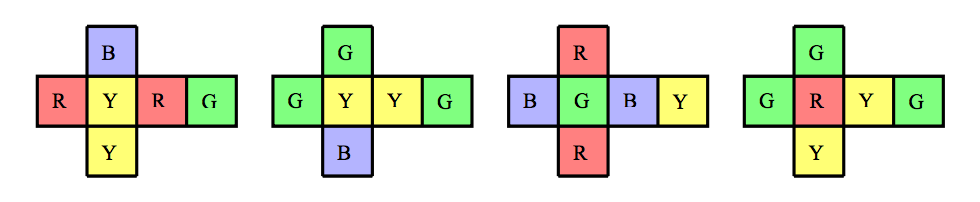
\includegraphics[width = .8\textwidth]{cubes.png}
	\end{center}
(Note: These cubes are colored differently than the ones from class.) Find a way to
stack all four cubes so that all four colors appear on each side of the resulting stack.

	\item Use induction to prove that the following formula holds for all $n \in \mathbb Z_{n>1}$:
	\[
		2 + 4 + 8 + 16 + 32 + \ldots + 2^n = 2^{n+1} - 2.
	\]

	\item A store offers gift card in the amounts of \$15 and \$25. What amounts can be made
using gift cards of these two types? Decide on an answer and then prove your answer
using induction.

\end{enumerate}





\end{document}